\chapter{How an Executor Uses Memory and CPU}
\label{ch:execmem}

\begin{chapterintro}
Spark runs on the Java Virtual Machine: the driver and every executor is a JVM
process, and the engine's memory behaviour, its failure modes, and much of its
internal design follow directly from how the JVM manages memory and runs code.
This chapter builds the memory map of a single executor --- which regions exist,
which a query can use, and which are consumed no matter what --- then adds the
two costs layered on top of it: garbage collection and serialization. By the end
you can size a pod from its configuration, explain a container kill that left no
Java error, and read GC time in the UI. How execution and storage memory borrow
from each other while a job runs is picked up alongside caching in
\Cref{ch:caching}; how to size these regions for a workload is \Cref{ch:tuning}.
\end{chapterintro}

\section{The JVM in one page: bytecode and just-in-time compilation}
\label{sec:mem-jvm}

Spark is written in Scala and runs on the Java Virtual Machine, and two features
of that platform shape how it performs.

The first is \emph{just-in-time compilation}. Spark's code is written in Scala,
and a processor cannot run Scala directly. Two translation steps stand between the
code and the processor.

The first step happens once, before anything runs. The Scala compiler turns the code
into \emph{bytecode}: a list of small, simple instructions that is the same on every
machine. The processor cannot run bytecode either, so the JVM must translate it
again, while the program is running.

The JVM has two ways to do that. It starts with an \emph{interpreter}, which reads
one bytecode instruction at a time and carries it out. That needs no preparation,
but it is slow. While it works, the JVM counts how often each piece of code (a
\emph{method}) is called. A method that is called again and again is \emph{hot}.
For hot methods the JVM switches to the second way. The \emph{just-in-time
compiler}, or JIT, translates the whole method once into \emph{machine code}, the
instructions the processor understands directly. Bytecode is not one long
sequence that the JVM walks through from the top. It is organized into methods, and
the JIT works one method at a time. Once method A has been compiled, every later
call to A skips the interpreter and runs A's machine code. Method B, which has not
been called often, is still interpreted, until it becomes hot and gets its own
machine code in turn.

Here is what that looks like for real. This small class is written in Java so it
is easy to read; the Scala compiler produces the same kind of bytecode. It mimics
the filter in the query below:

\begin{lstlisting}[language=Java,numbers=none,caption={A tiny class that mimics the filter in the query below},captionpos=b,label=lst:mem-java-source]
public class RowFilter {
    private double sum = 0.0;

    // called once per row
    boolean isLarge(double orderTotal) {
        return orderTotal > 100.0;
    }
    // called once per row above 100
    void addToSum(double orderTotal) {
        sum = sum + orderTotal;
    }
    // called once per row
    void processRow(double orderTotal) {
        if (isLarge(orderTotal)) {
            addToSum(orderTotal);
        }
    }
    // called once, at the end
    double result() {
        return sum;
    }
}
\end{lstlisting}

Compiling it and listing the bytecode with \texttt{javap -c -p} (JDK~18) gives the
following. Every unindented name is a method, and the numbered lines under it are
that method's bytecode instructions.

\begin{lstlisting}[language=text,numbers=none,caption={The bytecode of RowFilter, one block per method (constructor omitted)},captionpos=b,label=lst:mem-bytecode-methods]
boolean isLarge(double);
    0: dload_1
    1: ldc2_w        #13     // double 100.0d
    4: dcmpl
    5: ifle          12
    8: iconst_1
    9: goto          13
   12: iconst_0
   13: ireturn

void addToSum(double);
    0: aload_0
    1: aload_0
    2: getfield      #7      // Field sum:D
    5: dload_1
    6: dadd
    7: putfield      #7      // Field sum:D
   10: return

void processRow(double);
    0: aload_0
    1: dload_1
    2: invokevirtual #15     // Method isLarge:(D)Z
    5: ifeq          13
    8: aload_0
    9: dload_1
   10: invokevirtual #19     // Method addToSum:(D)V
   13: return

double result();
    0: aload_0
    1: getfield      #7      // Field sum:D
    4: dreturn
\end{lstlisting}

The class has four methods, and the \texttt{invokevirtual} lines in
\texttt{processRow} are the calls to the other two. Run it over the rows of the query.
\texttt{processRow} and \texttt{isLarge} run once per row, so they become hot
within the first few thousand rows. \texttt{addToSum} runs only for rows above 100,
so it becomes hot more slowly. \texttt{result} runs once, never becomes hot, and
stays interpreted for the whole job. Each method is judged and compiled on its own.

Think of a translator reading a speech aloud one sentence at a time. That is the
interpreter. When the same paragraph comes up again and again, the translator writes
out a finished translation once and reads from it. The first reading is slow and the
later ones are quick.

Here is what ``called again and again'' means in Spark. Take this query on the
lab's \texttt{orders} table, which has 30 million rows:

\begin{lstlisting}[language=sql,numbers=none,caption={A query whose inner step runs once per row},captionpos=b,label=lst:mem-hot-method]
SELECT sum(order_total)
FROM orders
WHERE order_total > 100;
\end{lstlisting}

\noindent An executor works through the rows one at a time. For every row it runs
the same small piece of code: read \texttt{order\_total}, compare it with 100, and if
it is larger, add it to the running sum. That piece of code is a method. The rows
change, but the method is the same, and it is called once per row, so 30 million
times. After a few thousand calls the JVM marks it hot and compiles it, and the
remaining millions of rows run the fast version. The same thing happens to every
step of a bigger query, such as the join and the grouping.
\Cref{fig:jvm-jit-pipeline} shows the path.

Two consequences matter for Spark. First, a Spark process is slowest in its first
seconds, before the JIT has found the hot methods. That is one reason interactive
sessions keep a driver alive instead of starting a new one for every query
(\Cref{sec:shape-deploy}), and why timing a snippet that runs only once tells you
almost nothing. Second, the JIT does its best work on simple, repetitive code, such
as a short loop that does the same thing to every row. It does less with code that
jumps between many different methods. That is why Spark's execution engine
generates one flat Java method for a chain of operators, instead of passing each row
from operator to operator (\Cref{sec:wholestage-codegen}, \Cref{ch:tungsten}).

\begin{figure}[H]
  \centering
  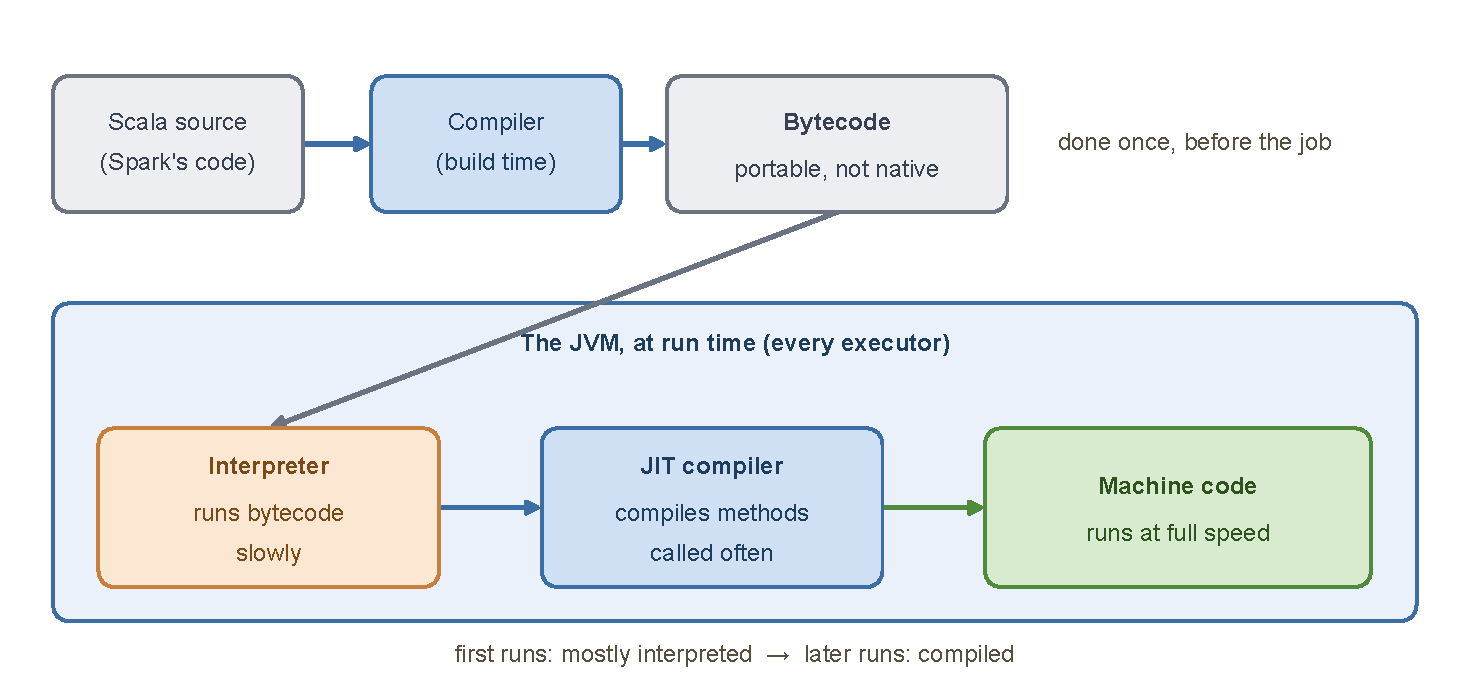
\includegraphics[width=0.95\linewidth]{jvm-jit-pipeline.pdf}
  \caption{From source to machine code. The compiler turns Scala into portable bytecode once. At run time the JVM starts by interpreting it, notices which methods are called often, and compiles only those to native code.}
  \label{fig:jvm-jit-pipeline}
\end{figure}

\paragraph{Reading the figure.} Follow the arrows from the top left.
\begin{enumerate}[nosep]
\item \textbf{Scala source} is the code the Spark developers wrote. The
      \textbf{compiler} runs once, at build time, and writes \textbf{bytecode}:
      instructions for an imaginary computer that look the same on every machine.
      Nothing has run yet.
\item Everything in the blue frame happens at run time, inside the JVM. The
      \textbf{interpreter} (orange, because it is the slow path) reads the bytecode
      and carries it out one instruction at a time. It can start at once, but it
      runs slowly.
\item While it interprets, the JVM counts how often each method is called. A method
      that is called often is \emph{hot}.
\item The \textbf{JIT compiler} translates only the hot methods into
      \textbf{machine code} (green, the fast path), which the processor runs
      directly. Later calls use that code.
\end{enumerate}
The line under the figure is the consequence: the first runs of a query are
mostly interpreted and slow, and later runs are mostly compiled and fast.


The lab measured the warm-up directly: the same filter-and-aggregate query run
eight times in one fresh JVM took 6.5~s the first time and 0.8--1.6~s from the
second run on (\Cref{fig:jit-warmup}) --- a factor of about eight, with nothing
changed but how much of the code the JIT had already compiled.

\begin{figure}[H]
  \centering
  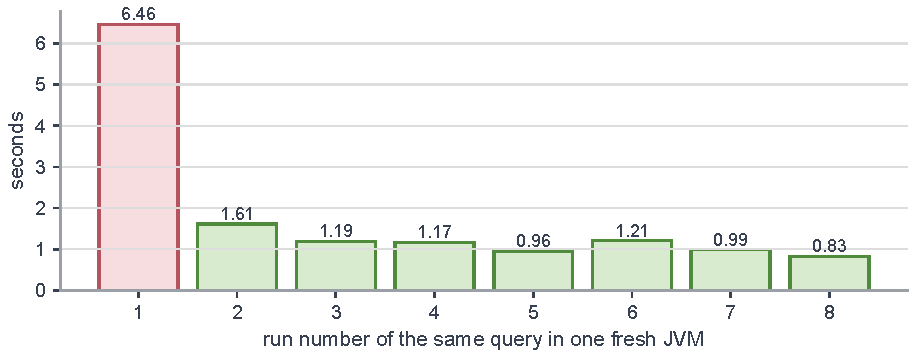
\includegraphics[width=0.9\linewidth]{jit-warmup.pdf}
  \caption{One query, eight consecutive runs in a fresh JVM. The first run pays
  for class loading, interpretation and compilation; later runs run compiled code.}
  \label{fig:jit-warmup}
\end{figure}

\paragraph{Reading the figure.} Each bar is one run of the same query. The horizontal axis counts
the runs, 1 to 8; the vertical axis is the time in seconds. The first bar (rose, the
cost) is 6.46~s: that run loads classes, interprets, and compiles. Bars 2 to 8
(green) are 0.83 to 1.61~s. Between run 1 and run 2 nothing changed except how much
of the code the JIT had already compiled.


The second is \emph{automatic memory management}: the program allocates objects
and never frees them, and a \emph{garbage collector} reclaims what is no longer
reachable. This is a convenience with a running cost, and for a data engine
moving billions of rows the cost is large enough that Spark works hard to keep
its data in a few large, packed buffers instead of millions of small objects,
which leaves the collector little to track. The rest of this
chapter is about where an executor's memory goes, and \Cref{sec:mem-gc} about
what the garbage collector does to it.

\section{Heap layout and object representation}
\label{sec:mem-heap}

The JVM manages a single contiguous region of memory, the \emph{heap}, from which
every object a program allocates is drawn. A Spark executor is one JVM process,
and the value of \conf{spark.executor.memory} is precisely the maximum size of
that heap. Everything a task does --- decoding a Parquet page into rows, building
a hash table for a join, accumulating a group-by result --- competes for space in
it, and when it fills, the task must either spill to disk or fail.

Two properties of the heap drive most of Spark's decisions about memory. The
first is \emph{per-object overhead}. Every object carries a header --- a mark word
and a pointer to its class --- before any field is stored, and the allocator pads
every object to an eight-byte boundary.

\begin{lstlisting}[numbers=none,caption={Cost of a boxed integer on a 64-bit JVM},captionpos=b,label=lst:mem-boxed-integer]
java.lang.Integer
  object header   12 bytes   (mark word + class pointer)
  int value        4 bytes
  ----------------------
  total           16 bytes   to carry 4 bytes of data
\end{lstlisting}

\noindent Measured with Spark's \texttt{SizeEstimator}, one million integers cost
4.0~MB as an \texttt{int[]} and 20.6~MB as a \texttt{List<Integer>}: 5.2 times
more (left panel of \Cref{fig:serialization-size}). A ten-character string
costs 56 bytes for 10 bytes of text. A row represented as an array of boxed Java objects (an
\texttt{Integer}, a \texttt{Double}, a \texttt{String} with its own header and
backing character array) can be several times larger in the heap than the same
row encoded as raw bytes. This is the amplification you see when a compressed
Parquet file expands to many times its on-disk size once decoded into Java
objects, and it is why Spark's execution engine stores rows in a packed binary format,
in a few large buffers, rather than as JVM objects (\Cref{ch:tungsten}).
\Cref{fig:object-overhead} shows where the extra bytes go.

\begin{figure}[H]
  \centering
  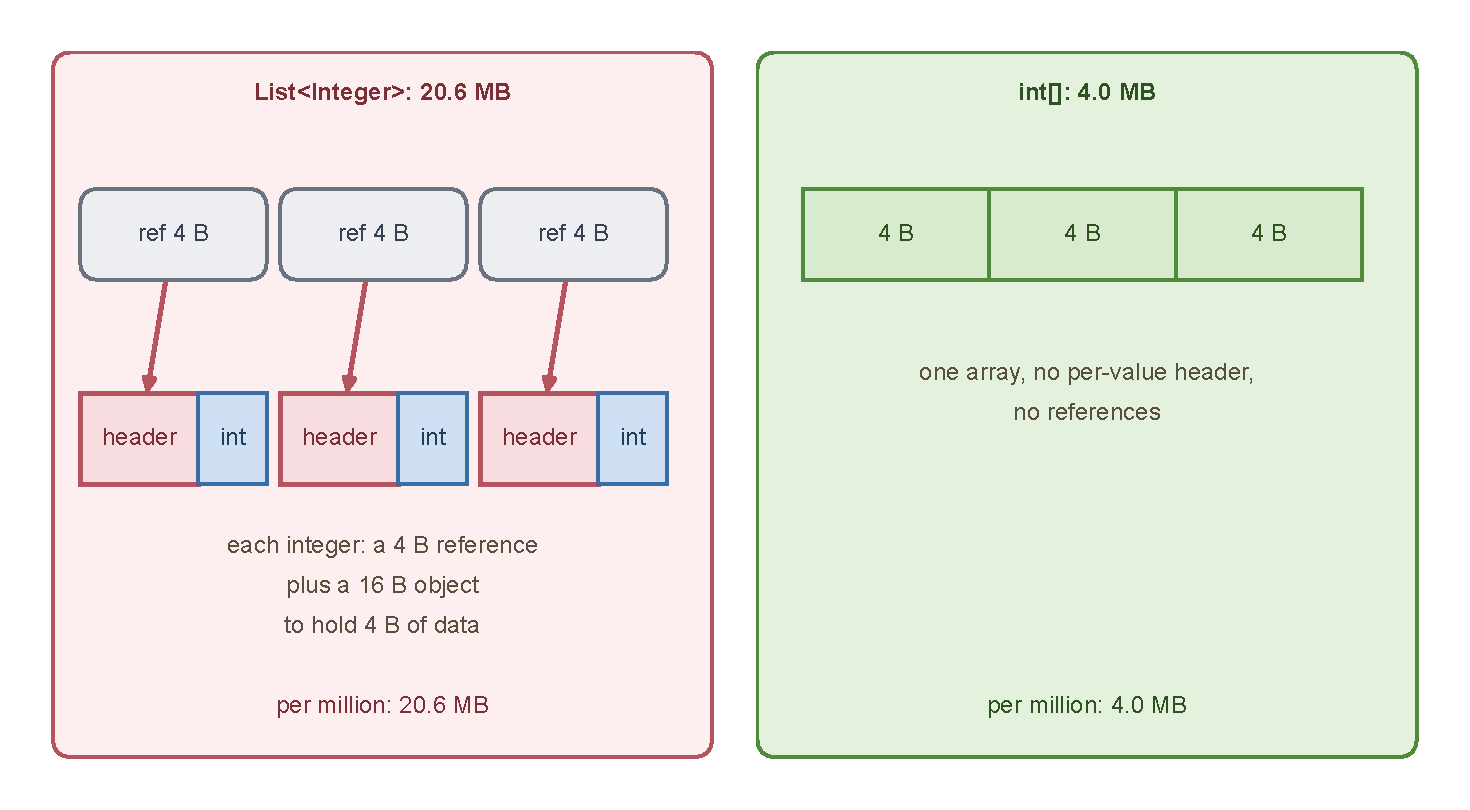
\includegraphics[width=0.95\linewidth]{object-overhead.pdf}
  \caption{One million integers, two layouts. A list of boxed integers pays a reference and an object header for every value; a primitive array stores only the values. The totals are the lab's measurements with Spark's \texttt{SizeEstimator}.}
  \label{fig:object-overhead}
\end{figure}

\paragraph{Reading the figure.} The two panels hold the same three numbers. The boxes are not drawn
to scale.
\begin{enumerate}[nosep]
\item \textbf{Left panel (rose, the costly layout).} The top row is the list. Each
      gray box is a 4-byte \emph{reference}: a pointer to an object stored somewhere
      else in memory. Each arrow leads to an \texttt{Integer} object, drawn in two
      pieces: the \emph{header} (rose) that every Java object carries, and the
      \texttt{int} value (blue), the only piece that is actual data. The object is
      16 bytes, 12 of them header and 4 of them value, as the listing above shows.
\item Adding it up: 4 bytes of reference plus a 16-byte object, about 20 bytes, to
      store 4 bytes of data.
\item \textbf{Right panel (green).} An \texttt{int[]} stores the 4-byte values
      side by side in one block. There are no references and no per-value header.
\item The bottom line of each panel is the lab's measurement for a million
      integers: 20.6~MB against 4.0~MB.
\end{enumerate}


The second property is that the heap is \emph{managed}: the program never frees
memory explicitly, and reclamation is the job of the garbage collector
(\Cref{sec:mem-gc}). Spark does not hand the whole heap to a query; it subdivides
it into regions with different owners and different rules, described next.

\section{The executor memory model}
\label{sec:mem-model}

Configuring Spark's memory means deciding how one executor process divides the
memory it is allowed to use. That memory has three separately configured
parts: the heap, an optional off-heap pool, and overhead. The heap is itself
divided into reserved, unified, and user memory. Confusing these is the most
common source of both wasted memory and unexplained container kills.

\begin{analogy}
Picture the heap as an apartment building with a fixed number of floors
(\conf{spark.executor.memory}). One utility closet is permanently locked for
building systems (\emph{reserved}) --- no tenant ever gets a key. A shared
common floor (\emph{unified memory}) is reconfigured on demand: some nights it
hosts a big event that needs the whole floor (\emph{execution}), other nights
it is rented out as storage lockers (\emph{storage}) --- and management can
always cancel a storage booking to make room for a scheduled event, but never
the reverse. The remaining floors are private apartments (\emph{user memory}):
whatever a tenant does inside their own apartment is invisible to the building
manager, and if a tenant packs it past capacity, nobody bails them out --- the
apartment simply collapses (\conf{OutOfMemoryError}). A separate storage unit
down the street, rented by some tenants but not others, is the \emph{off-heap}
pool; and the building's own infrastructure --- elevators, wiring, hallway
lighting (\emph{overhead}) --- draws power regardless of occupancy. The whole
lot only fits inside the property line the landlord (the cluster manager)
enforces: exceed it, and the building is condemned, tenants and all.
\end{analogy}

\Cref{fig:executor-memory-model} is the whole map in one picture. The paragraphs after it take it apart piece by piece.

\begin{figure}[H]
  \centering
  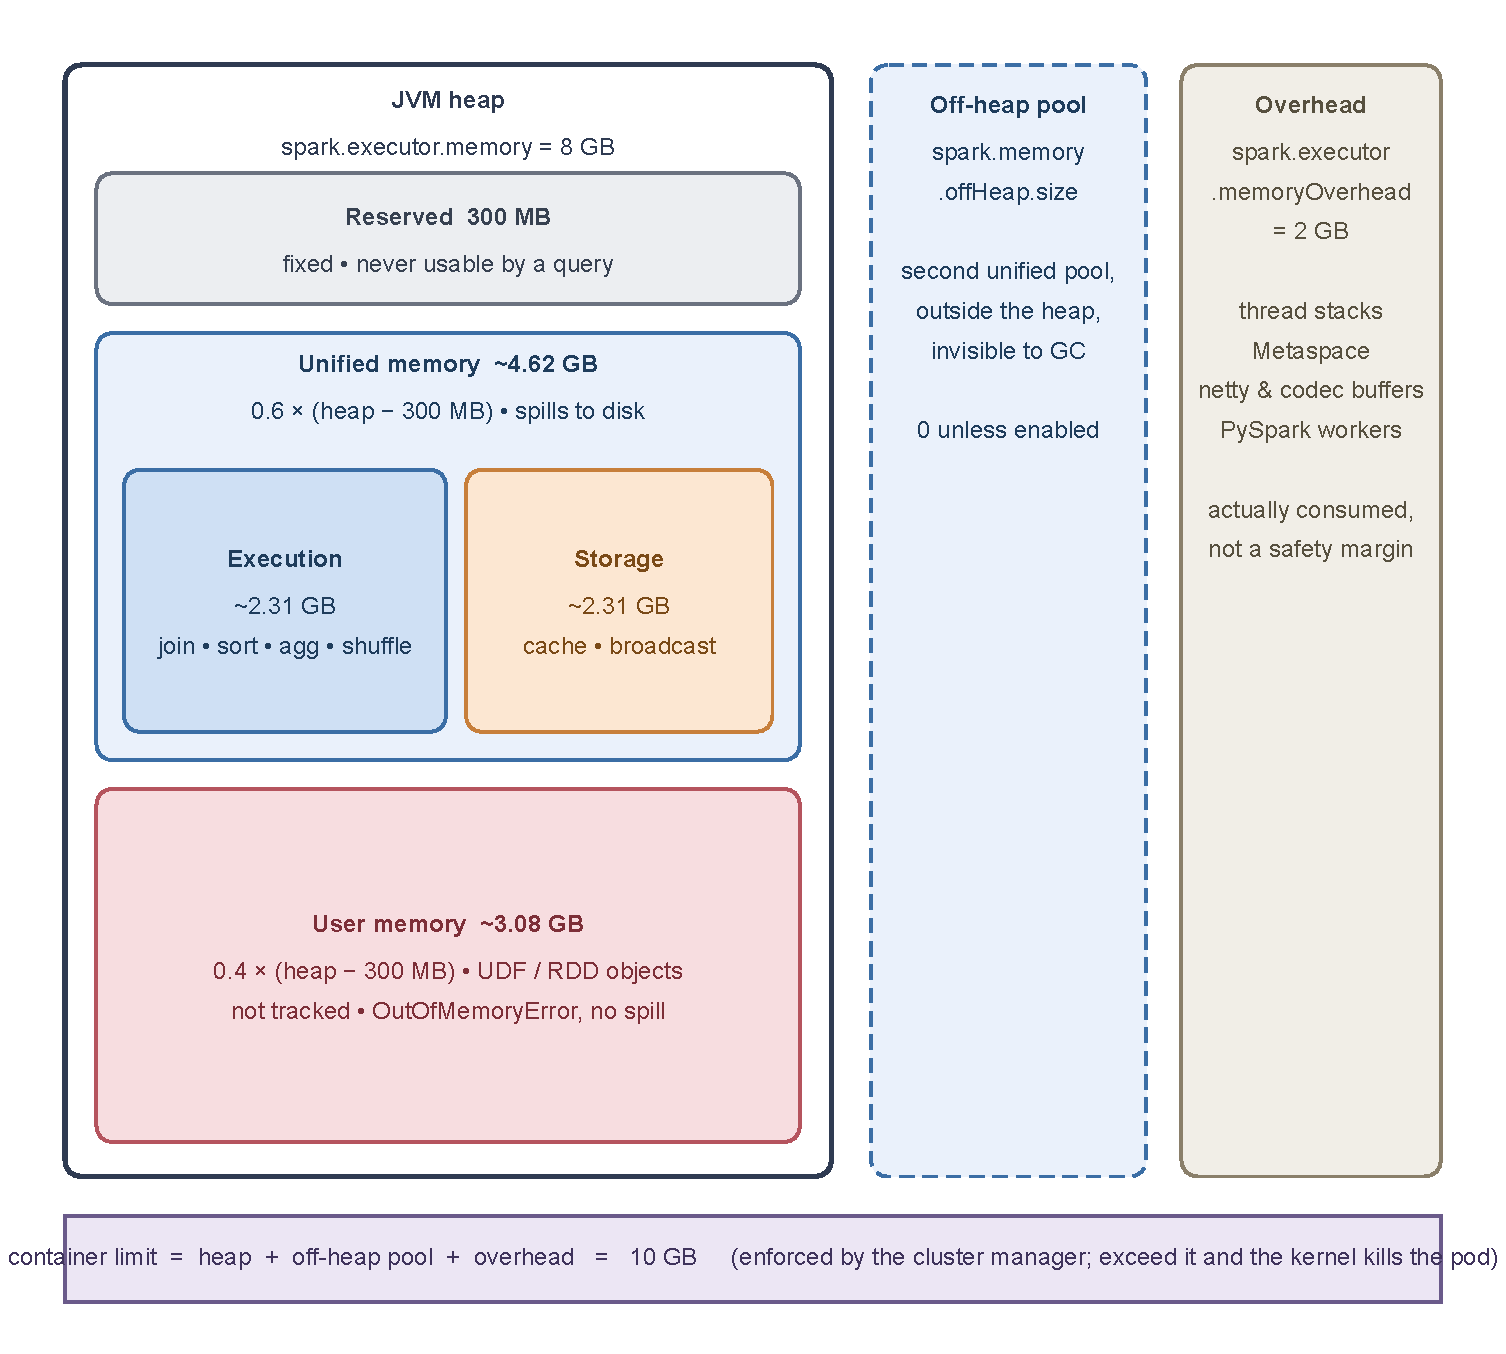
\includegraphics[width=\linewidth]{executor-memory-model.pdf}
  \caption{An executor's memory: the JVM heap (reserved / unified / user), the
  optional off-heap pool, and the overhead the process needs outside both. The
  cluster manager's container limit must cover all three. Numbers are worked for
  an 8~GB heap with 2~GB overhead.}
  \label{fig:executor-memory-model}
\end{figure}

\paragraph{Reading the figure.} The figure works through an example with an 8~GB heap and 2~GB of
overhead. Read it left to right.
\begin{enumerate}[nosep]
\item \textbf{JVM heap} (the large frame on the left) is everything
      \conf{spark.executor.memory} sets. From the top: \textbf{Reserved} (gray) is a
      fixed 300~MB that no query can use. \textbf{Unified memory} (blue) is about
      4.6~GB, $0.6 \times (\text{heap} - 300~\text{MB})$. It is the only pool Spark
      counts byte by byte, and the only one that spills to disk when full. It holds
      two shares of about 2.3~GB each, \textbf{Execution} (joins, sorts,
      aggregations, shuffle buffers) and \textbf{Storage} (cached and broadcast
      blocks), separated by a soft boundary. \textbf{User memory} (rose) is the
      remaining 40\%, about 3.1~GB, for the objects your own code creates. Spark
      neither counts nor spills it, so overflowing it ends in an
      \conf{OutOfMemoryError}.
\item \textbf{Off-heap pool} (dashed frame, middle) is a second unified pool
      outside the heap, sized by \conf{spark.memory.offHeap.size}. It is zero unless
      you enable it, which is why the frame is dashed.
\item \textbf{Overhead} (right) is 2~GB here. It covers thread stacks, class
      metadata, network and codec buffers, and PySpark worker processes. It is
      memory the process actually uses, not a safety margin.
\item \textbf{Container limit} (purple bar, bottom) is the sum of the three:
      heap, off-heap, and overhead, 10~GB in this example. The cluster manager
      enforces it from outside the JVM. If the process crosses it, the kernel kills
      the pod and no Java error appears.
\end{enumerate}

\paragraph{The heap.} \conf{spark.executor.memory} sets the maximum size of the
JVM heap, the region every object the executor allocates comes from. Spark carves
it into three parts:

\begin{itemize}
  \item \textbf{Reserved memory} --- a fixed 300~MB Spark holds back for its own
        internal objects. It is not configurable and never available to a query.
  \item \textbf{Unified memory} --- by default 60\% of (heap $-$ 300~MB), set by
        \conf{spark.memory.fraction}. This is the only pool Spark accounts for
        byte by byte and the only one that spills to disk gracefully when it runs
        out. It is shared between \emph{execution memory} (the working memory of a
        running operator: hash tables for joins and aggregations, sort buffers,
        the shuffle write buffer) and \emph{storage memory} (cached DataFrame and
        RDD blocks, and broadcast data held on the executor).
        \conf{spark.memory.storageFraction} (default 0.5) is a soft boundary
        between the two: either side may borrow the other's idle space. Execution
        can evict cached blocks only while storage holds more than its
        \conf{spark.memory.storageFraction} share; storage can never evict
        execution memory, so execution that has borrowed idle storage space keeps it
        until the task finishes. How this plays out while a job runs is covered in
        \Cref{ch:caching}.
  \item \textbf{User memory} --- the remaining 40\%. Everything Spark does not
        manage lives here: the objects your UDFs and RDD closures create, the
        structures a \texttt{mapPartitions} builds up. Spark does not track this
        pool and cannot spill it; overflowing it throws
        \conf{OutOfMemoryError} and kills the executor.
\end{itemize}

\paragraph{Off-heap memory.} When \conf{spark.memory.offHeap.enabled} is set,
\conf{spark.memory.offHeap.size} adds a second unified-memory pool that lives
outside the heap, addressed directly by the engine and invisible to the garbage
collector (\Cref{sec:mem-gc}). Execution and storage draw on it in addition to
their on-heap pool. It is not taken out of \conf{spark.executor.memory}; it is
additional memory the process reserves, and it must be counted into the
container's limit.

Concretely: an executor already running \conf{spark.executor.memory=8g} that
adds \conf{spark.memory.offHeap.enabled=true} and
\conf{spark.memory.offHeap.size=4g} does not shrink its 8~GB heap down to make
room for those 4~GB --- the 4~GB is layered on top, for a combined 12~GB of
heap plus off-heap unified memory before overhead is even added. The
container or pod limit has to be resized to cover all 12~GB (plus overhead)
or the extra off-heap pool simply causes the kind of container kill
\Cref{sec:failure-signatures} describes, with nothing in the JVM's own heap
metrics hinting at why.

\paragraph{Overhead.} \conf{spark.executor.memoryOverhead} (default the larger
of 384~MB and 10\% of the heap) is memory the process needs that is neither heap
nor off-heap pool: JVM thread stacks, class metadata (Metaspace), buffers for
network transfer and compression codecs, and --- for PySpark --- the Python
worker processes, which can each take hundreds of megabytes. It is not a safety
margin; it is space that is actually consumed, and its default is frequently too
small for PySpark or codec-heavy workloads, in which case the container is killed
with no Spark-level error.

\paragraph{The pool, measured.} The lab read the unified pool from Spark's memory
manager for four heap sizes (\Cref{tab:mem-pool-measured}); the formula
$(\text{heap} - 300~\text{MiB}) \times 0.6$ matches to the decimal. The reserved
300~MiB also sets a floor: asked to start with a 400~MB heap, Spark refused with
\texttt{[INVALID\_DRIVER\_MEMORY] System memory 405471232 must be at least
471859200} --- 450~MiB, which is 1.5 times the reserved amount.

\begin{table}[htbp]
\centering\footnotesize
\renewcommand{\arraystretch}{1.2}
\begin{tabular}{@{}rrr@{}}
\toprule
\textbf{Heap (\conf{-Xmx})} & \textbf{Unified pool, measured (MiB)} & \textbf{$(\text{heap} - 300) \times 0.6$ (MiB)} \\
\midrule
512 MiB & 127.2 & 127.2 \\
1 GiB & 434.4 & 434.4 \\
2 GiB & 1048.8 & 1048.8 \\
4 GiB & 2277.6 & 2277.6 \\
\bottomrule
\end{tabular}
\caption{The unified pool against the formula, on four heaps (Spark 3.5.2).}
\label{tab:mem-pool-measured}
\end{table}

\paragraph{What the cluster manager enforces.} The pod or container is sized as
the sum of all three pools (\Cref{fig:executor-memory-model}). If the process's
real usage crosses that limit --- most often because overhead was underestimated
or off-heap memory was not counted into the limit --- the kernel kills it
(\Cref{sec:failure-signatures}). The heap merely filling up, by contrast, makes
unified memory spill to disk and only throws when user memory or a single
un-spillable allocation is the cause.

\paragraph{Per task, not per executor.} Execution memory is shared by the tasks an
executor runs at the same moment, one per core (\conf{spark.executor.cores}). Adding
cores to the same heap therefore shrinks each task's share: memory per task is the
pool divided by the core count. \Cref{fig:memory-per-task} works it through for the
4~GiB heap of \Cref{tab:mem-pool-measured}: the 2,278~MiB pool gives each of 4 tasks
about 569~MiB and each of 8 tasks about 285~MiB. The number of cores per executor is
therefore a memory decision as much as a parallelism one, and an executor with too
many cores spills on work a narrower one finishes in memory.
\Cref{fig:spill-heatmap} measured exactly this on twelve executor shapes
(\Cref{sec:executor-sizing}).

\begin{figure}[H]
  \centering
  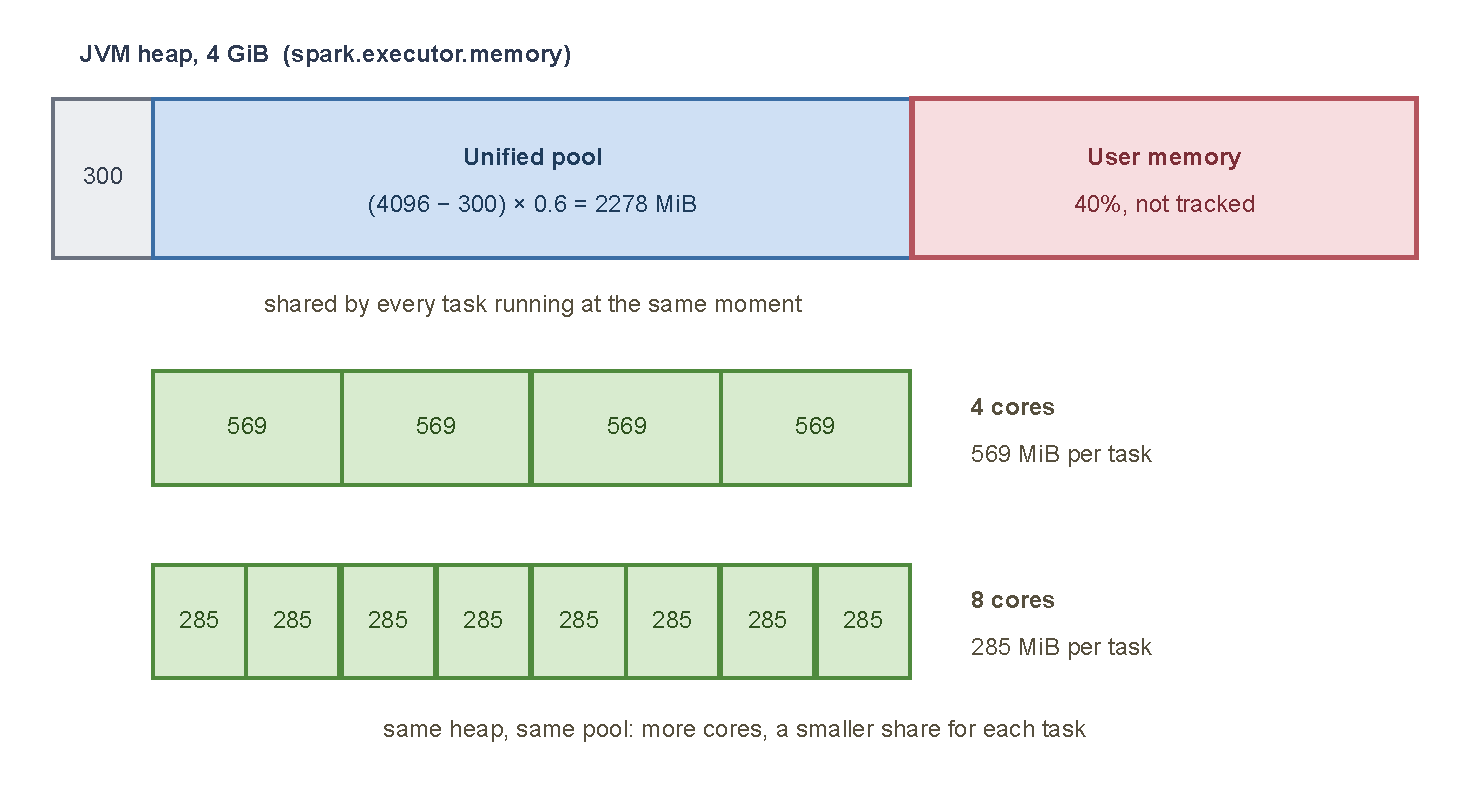
\includegraphics[width=0.95\linewidth]{memory-per-task.pdf}
  \caption{From heap to a task's share, for a 4~GiB heap. The unified pool is shared by every task that runs at the same moment, so doubling the cores halves each task's room. The numbers inside the green boxes are MiB per task.}
  \label{fig:memory-per-task}
\end{figure}

\paragraph{Reading the figure.} Read it from the top.
\begin{enumerate}[nosep]
\item \textbf{The bar on top} is the 4~GiB heap, drawn to scale. The gray
      sliver on the left is the 300~MiB reserve. The blue part is the unified
      pool, $(4096 - 300) \times 0.6 = 2278$~MiB. The rose part is user memory, the
      other 40\%, which Spark does not track.
\item \textbf{The green row marked ``4 cores''} splits the blue pool among the four
      tasks that run at the same moment. Each box is one task's share: $2278 \div 4
      \approx 569$~MiB.
\item \textbf{The row marked ``8 cores''} splits the same pool eight ways:
      $2278 \div 8 \approx 285$~MiB each.
\item The pool did not grow between the rows. Only the number of tasks sharing it
      did. A task that needs 400~MiB for a sort fits in the first row and spills in
      the second; \Cref{ch:tuning} measures how much a real stage needs.
\end{enumerate}


\section{Garbage collection: Parallel, G1, ZGC}
\label{sec:mem-gc}

Because the heap is managed, the JVM must periodically find objects that are no
longer reachable and reclaim their space. This work is the \emph{garbage
collector} (GC), and for a data-processing workload it is never free: the
collector competes with the application for CPU, and some of its phases are
\emph{stop-the-world}, meaning every application thread in the JVM is frozen until
the phase completes (\Cref{fig:gc-pause-stall}). On an executor a long stop-the-world pause stalls every
running task at once, and if it exceeds the heartbeat timeout the driver declares
the executor lost and re-runs its work elsewhere (\Cref{sec:failure-signatures}).

Collectors differ mainly in how they trade pause length against throughput and
CPU cost. \Cref{fig:gc-collector-timelines} sketches the pause pattern of each.

\begin{figure}[H]
  \centering
  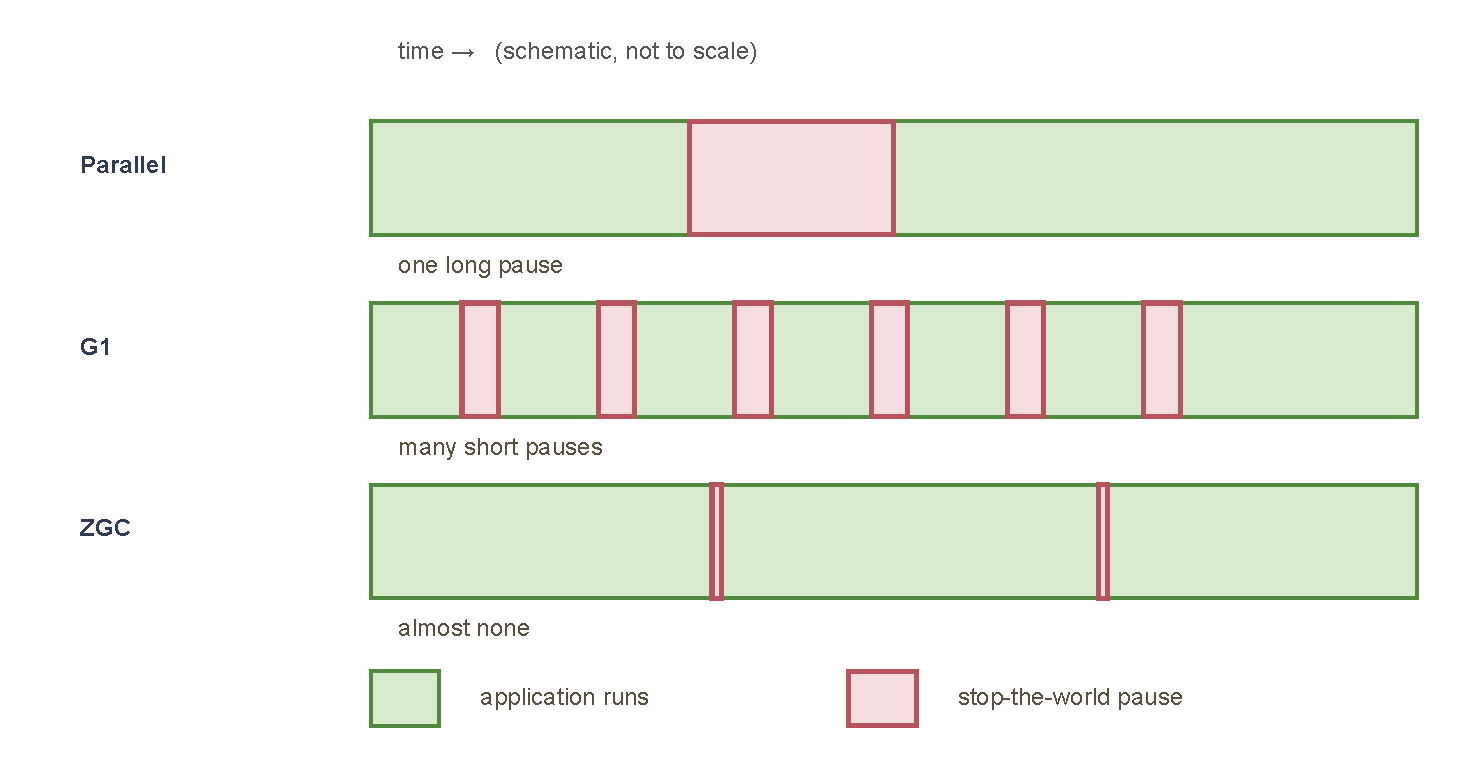
\includegraphics[width=0.95\linewidth]{gc-collector-timelines.pdf}
  \caption{Pause shapes of the three collectors on the same timeline. Green is the application running; rose is a stop-the-world pause. The sketch shows the pattern, not measured values; the measurements follow in \Cref{fig:gc-collectors-measured}.}
  \label{fig:gc-collector-timelines}
\end{figure}

\paragraph{Reading the figure.} Each row is one collector over the same stretch of time. Green is
the application running. Rose is a stop-the-world pause, when every application
thread is frozen.
\begin{enumerate}[nosep]
\item \textbf{Parallel} has one long pause: it collects the whole heap at once.
\item \textbf{G1} has many short pauses: each one collects a small slice of the heap.
\item \textbf{ZGC} has almost no pauses: it does its work while the application
      runs, at the price of more CPU.
\end{enumerate}
The widths are a sketch, not measured. The next figure gives the measured
values for the lab's stage.


\begin{analogy}
Picture three ways to clean a large office building overnight. Parallel GC is
an all-lights-off deep clean: every employee is sent home, the whole crew
cleans the whole floor at once, and the doors reopen only when they are
finished --- the fastest total clean, but nobody works while it happens. G1
cleans one wing at a time while the rest of the building stays open, closing
only the wing being cleaned right now, briefly and often. ZGC has cleaners who
tidy around the working employees continuously and almost invisibly, closing
nothing at all --- at the cost of moving more carefully and needing a bigger
crew.
\end{analogy}

\begin{itemize}
  \item \textbf{Parallel GC} uses multiple threads but collects the whole heap in
        one stop-the-world pause. It gives the highest raw throughput when pauses
        do not matter, but pause time grows with heap size, so a large executor
        can freeze for seconds at a time.
  \item \textbf{G1} (Garbage-First) divides the heap into equal-sized regions and
        collects a subset of them per cycle, doing most of its marking
        concurrently with the application. Pause times are shorter and roughly
        bounded regardless of heap size, at the cost of more bookkeeping and CPU.
        It is the default at the heap sizes a Spark executor typically runs and
        the collector most Spark tuning assumes.
  \item \textbf{ZGC} does essentially all of its work concurrently and keeps
        pauses under a millisecond even on very large heaps, at a higher constant
        CPU and memory overhead. It is worth choosing only for executors with
        tens of gigabytes of heap where G1 pauses are still a problem.
\end{itemize}

\begin{table}[H]
\centering\footnotesize
\renewcommand{\arraystretch}{1.25}
\begin{tabular}{@{}P{1.8cm}P{3.4cm}P{3.6cm}P{5cm}@{}}
\toprule
\textbf{Collector} & \textbf{Pause} & \textbf{Throughput / CPU} & \textbf{Best for} \\
\midrule
Parallel & long, grows with heap & highest throughput, lowest overhead & batch jobs where pauses don't matter \\
G1 (default) & short, roughly bounded & moderate bookkeeping cost & most Spark executors \\
ZGC & sub-millisecond & higher constant CPU \& memory & very large heaps where G1 still pauses \\
\bottomrule
\end{tabular}
\caption{The three collectors, at a glance.}
\label{tab:mem-collectors}
\end{table}

\begin{figure}[H]
  \centering
  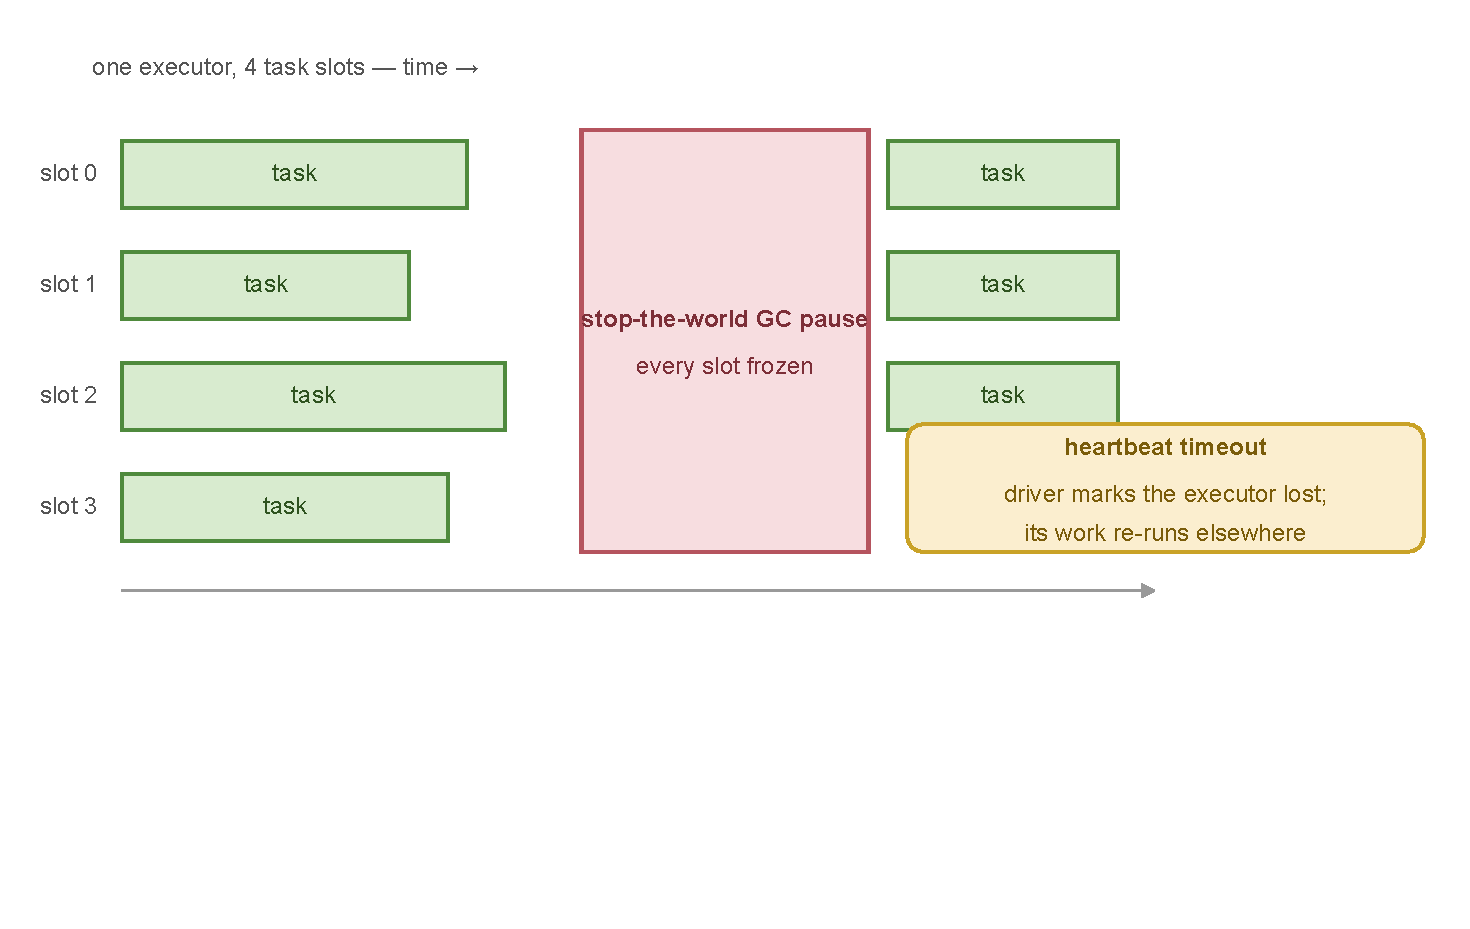
\includegraphics[width=\linewidth]{gc-pause-stall.pdf}
  \caption{A stop-the-world pause freezes every task slot on the executor at
  once, not one at a time. If the pause outlasts the heartbeat timeout
  (\conf{spark.network.timeout}, 120~s by default), the
  driver concludes the executor is gone and re-runs its work elsewhere --- so a
  GC problem shows up as lost executors and repeated stages, not just as slow
  ones.}
  \label{fig:gc-pause-stall}
\end{figure}

\paragraph{Reading the figure.} Time runs from left to right. Each row is one of the four task slots
of a single executor, and each green bar is a task running in that slot.
\begin{enumerate}[nosep]
\item The tall rose block in the middle is a stop-the-world pause. It covers
      \emph{all four rows at once}, because the pause freezes the whole JVM, not one
      task. The tasks to its left stop where they are; the green bars to its right
      are the same slots getting back to work.
\item The amber box at the bottom shows what happens if the pause is long. The
      executor cannot send its heartbeat while it is frozen. If it stays silent past
      the timeout, the driver marks the executor lost and re-runs its work elsewhere.
\item That is why a GC problem can show up as lost executors and repeated stages,
      not only as slow ones.
\end{enumerate}


The lab ran the same sort-heavy stage (4~GB heap, 8 cores) under each collector
(\Cref{fig:gc-collectors-measured}). Wall-clock time was within 1.3 seconds for G1
and Parallel (22.8 and 23.1~s) and 19\% worse for ZGC (27.2~s). The pauses differ
sharply: G1 paused 118 times for 574~ms in total, its longest pause 47~ms; Parallel
paused 38 times for 3.4~s in total, its longest 835~ms. The \emph{GC time} column of
the task metrics shows something the pause log does not: 1.8~s for G1 but 25.4~s for
Parallel, because the metric is accumulated \emph{per task}, so one stop-the-world
pause is counted once for every task that was running through it --- 835~ms across
eight slots is nearly seven seconds. (ZGC's 34.5~s is concurrent collector work
charged to tasks; the lab's \texttt{-Xlog:gc} format for ZGC carries no pause
lines, so its pause column is not available.) On this stage, at a 4~GB heap, G1's
shorter pauses cost no throughput and ZGC cost throughput.

\begin{figure}[H]
  \centering
  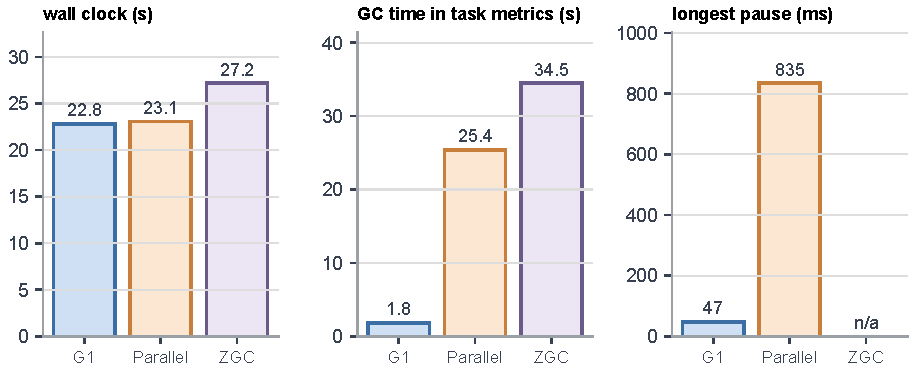
\includegraphics[width=\linewidth]{gc-collectors-measured.pdf}
  \caption{One stage under three collectors. Wall clock is close for G1 and
  Parallel; the longest pause and the per-task GC metric are not.}
  \label{fig:gc-collectors-measured}
\end{figure}

\paragraph{Reading the figure.} There are three panels, one per measurement, and the same three
collectors in each: G1 (blue), Parallel (orange), and ZGC (purple).
\begin{enumerate}[nosep]
\item \textbf{Wall clock (left)} is how long the stage took: 22.8, 23.1 and
      27.2~s. G1 and Parallel are close; ZGC is slower.
\item \textbf{GC time in task metrics (middle)} is the GC time summed over all
      tasks: 1.8, 25.4 and 34.5~s. It is far larger than the pause time because each
      task counts a pause that happened while it was running.
\item \textbf{Longest pause (right)} is the single worst freeze: 47~ms for G1 and
      835~ms for Parallel. ZGC shows ``n/a'' because the lab's log format for ZGC
      has no pause lines.
\end{enumerate}


The generational hypothesis --- that most objects die young --- underlies Parallel
GC and G1: they collect a small ``young'' area cheaply and often, and the full heap
rarely (\Cref{fig:gc-generations}). ZGC on JDK~17 is not generational; generational
ZGC arrives in JDK~21. A workload that holds a large amount of long-lived data in
cache violates the hypothesis and pushes the collector toward the expensive path,
which is one more reason to cache deliberately (\Cref{ch:caching}).

\begin{figure}[H]
  \centering
  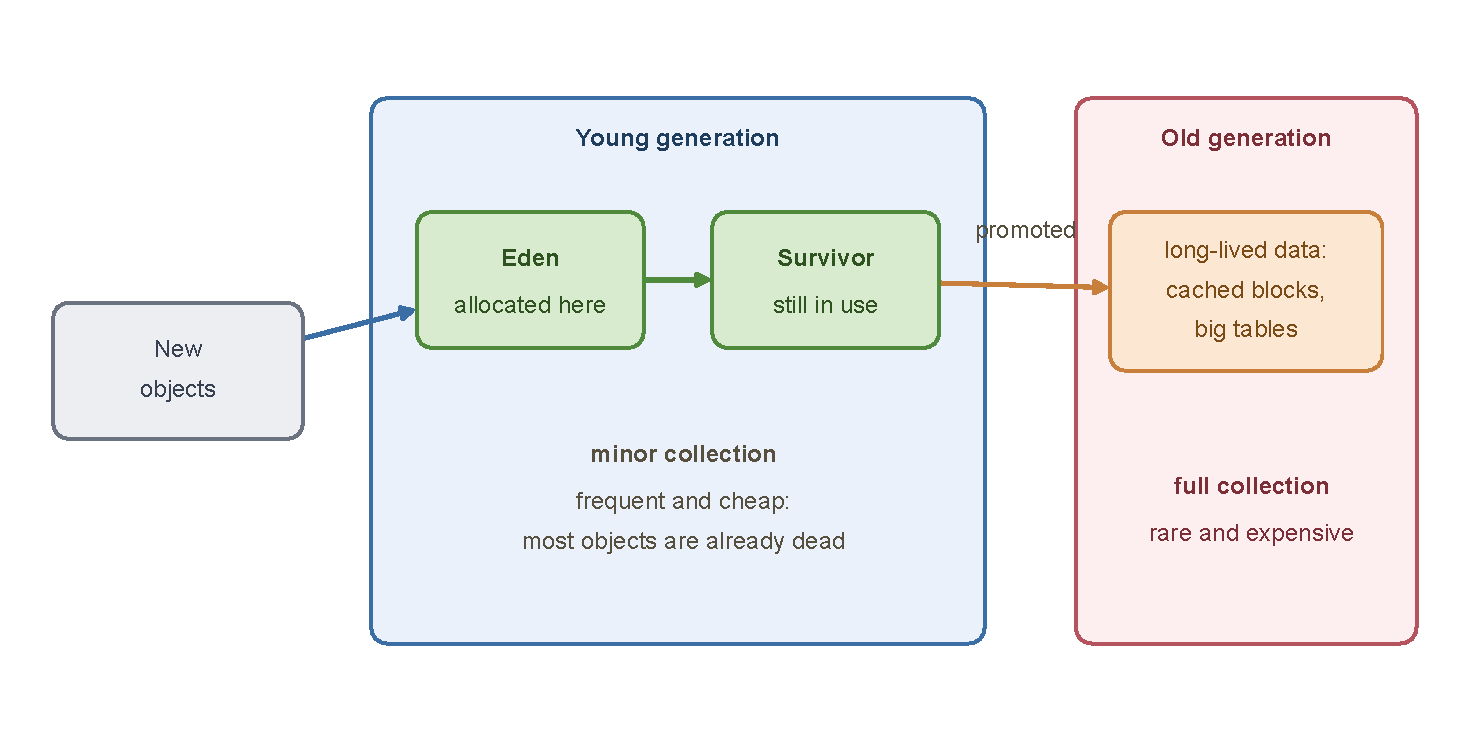
\includegraphics[width=0.95\linewidth]{gc-generations.pdf}
  \caption{The generational layout used by Parallel GC and G1. New objects start in the young generation, where most die quickly and a minor collection is cheap. Objects that survive repeatedly are promoted to the old generation, which only a full collection cleans.}
  \label{fig:gc-generations}
\end{figure}

\paragraph{Reading the figure.} Follow the arrows from the left.
\begin{enumerate}[nosep]
\item \textbf{New objects} (gray) are allocated in \textbf{Eden}, the first
      area of the young generation.
\item When Eden fills, a \emph{minor collection} runs. It copies the objects that
      are still in use into a \textbf{Survivor} area and frees everything else in one
      step. It is cheap because most objects are already dead, so there is little to
      copy.
\item An object that survives several minor collections is \emph{promoted} (the
      orange arrow) to the \textbf{old generation}. That frame is rose because
      cleaning it is the costly operation.
\item The old generation fills slowly. When it is full a \emph{full collection}
      has to examine a large part of the heap: rare, but long.
\end{enumerate}
This matters for Spark because cached blocks and big hash tables live a long time.
They pile up in the old generation and make full collections more likely.


Monitoring GC time is covered in \Cref{sec:reading-metrics}; the executor JVM
options that select and tune a collector are in \Cref{ch:tuning}.

\section{Serialization and its cost}
\label{sec:mem-serialization}

The engine keeps a join's hash table or a block of cached rows in a few large
byte buffers rather than millions of small Java objects, so the garbage collector
has little to track (\Cref{sec:mem-model}, \Cref{ch:tungsten}). Getting
data into and out of that flat form is serialization.

\emph{Serialization} is the conversion of an in-memory object graph into a flat
sequence of bytes, and \emph{deserialization} is its inverse. Spark serializes
whenever data leaves a JVM: across the network during a shuffle, to disk when
unified memory spills or a block is cached in serialized form, and when a
broadcast variable is shipped to executors. The cost is both CPU and size.

The two options for arbitrary Java objects differ sharply. The built-in Java
serializer writes the full class name and every field name and type alongside the
values, repeated for every object, so most of the output is self-description
rather than data. \emph{Kryo} writes a compact encoding --- a short numeric class
identifier and the field values. The lab serialized 20,000 five-field records
both ways (right panel of \Cref{fig:serialization-size}): one record at a time,
Java wrote 299 bytes per record and Kryo 42 --- seven times smaller; as one array
the gap shrinks to 58 against 41 bytes per record, because the class description is
written once. The advantage is therefore largest for many small separately
serialized objects, which is what a shuffle of RDD records is.
\Cref{fig:serialization-bytes} shows why.

\begin{figure}[H]
  \centering
  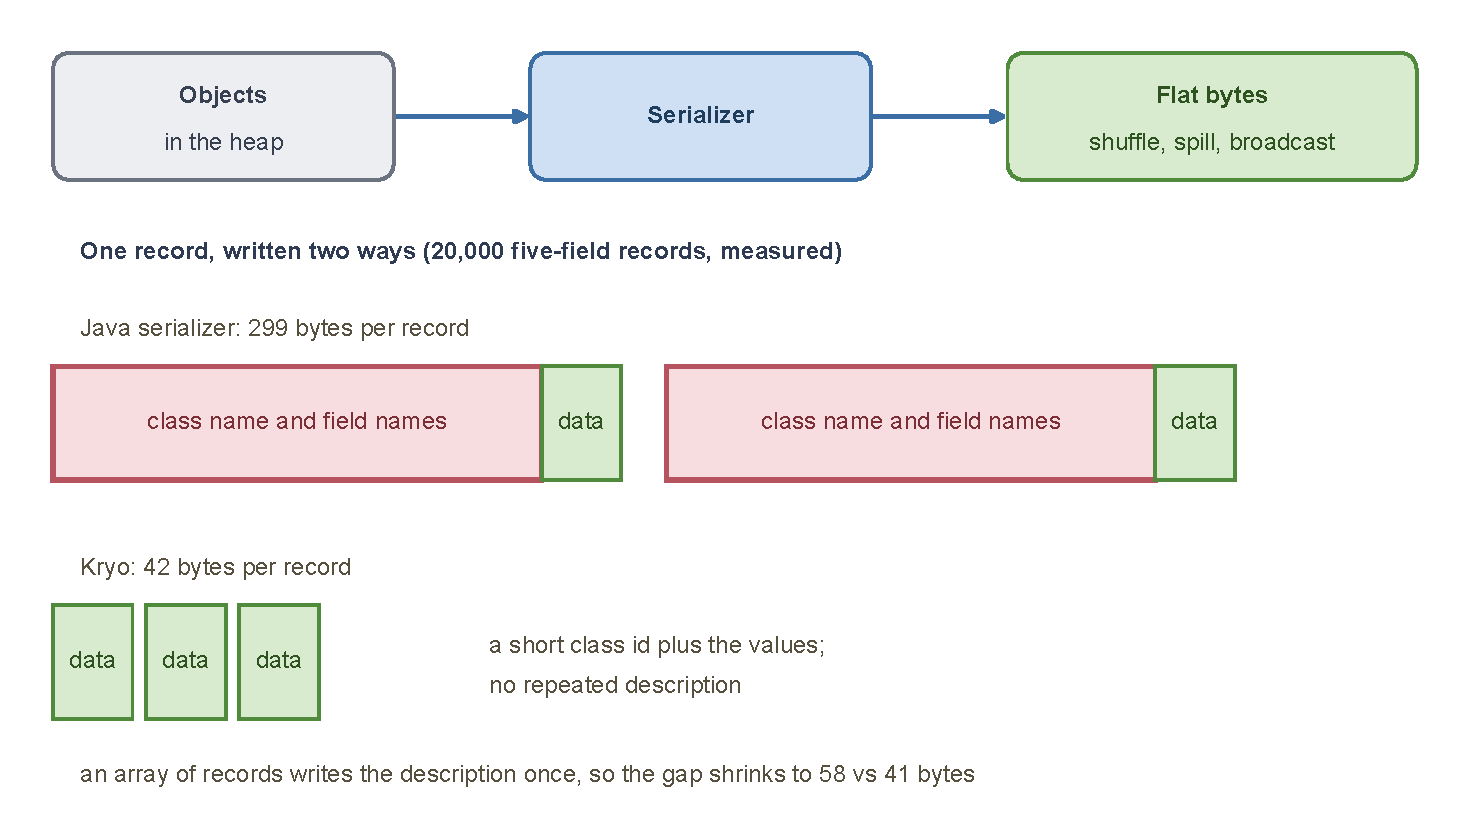
\includegraphics[width=0.95\linewidth]{serialization-bytes.pdf}
  \caption{What a serializer does, and why Kryo is smaller. Java writes the class and field names with every record; Kryo writes a short class id and the values. Sizes are the lab's measurement for one five-field record.}
  \label{fig:serialization-bytes}
\end{figure}

\paragraph{Reading the figure.} The picture has two parts.
\begin{enumerate}[nosep]
\item \textbf{The top row} shows what a serializer is for. Objects in the heap
      (gray) go through the serializer (blue) and come out as flat bytes (green).
      Flat bytes can leave the JVM: they can be shuffled, spilled to disk, or
      broadcast.
\item \textbf{The lower part} shows one five-field record written two ways, with
      widths proportional to the number of bytes. In the Java row, every record is a
      rose block (the class name and field names) followed by a small green block
      (the data). Two records are shown, so the rose block appears twice. In the
      Kryo row there is only data, and three records take up less room than one
      Java record: 42~bytes each against 299.
\item The last line explains the exception. When the whole array of records is
      written at once, Java writes the class description a single time, and the gap
      shrinks to 58 against 41~bytes per record.
\end{enumerate}


\begin{figure}[H]
  \centering
  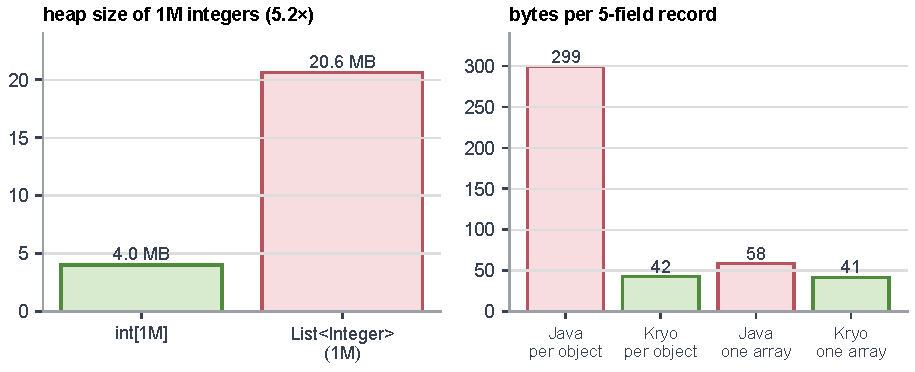
\includegraphics[width=\linewidth]{serialization-size.pdf}
  \caption{Left: one million integers as a primitive array and as boxed objects.
  Right: bytes per five-field record under Java and Kryo serialization, one record
  at a time and as one array.}
  \label{fig:serialization-size}
\end{figure}

\paragraph{Reading the figure.} The figure has two panels.
\begin{enumerate}[nosep]
\item \textbf{Left panel:} the heap size of one million integers. The green bar
      is the primitive array, 4.0~MB. The rose bar is the list of boxed objects,
      20.6~MB: 5.2 times more, for the same values.
\item \textbf{Right panel:} the bytes needed to write one five-field record, in four
      cases. Rose bars are the costly ones. Java writing one record at a time takes
      299~bytes and Kryo 42. Writing the whole array in one go takes Java 58~bytes
      per record and Kryo 41, because the class description is written once.
\end{enumerate}


The smaller output directly reduces shuffle volume, spill size and broadcast
footprint (\Cref{ch:tuning}).

DataFrame and SQL workloads sidestep both serializers for most operations: rows
already live in the engine's binary format (\Cref{ch:tungsten}), so moving them
is a memory copy with no object graph to walk. The Java-versus-Kryo choice still
governs RDD code, user-defined functions, and anything that puts arbitrary Java
objects into a shuffle or a broadcast --- the same user-memory objects that
\Cref{sec:mem-model} noted Spark does not manage.

\section{Summary}
\label{sec:mem-summary}

An executor is one JVM process, and its memory is three separately configured
parts: the heap (\conf{spark.executor.memory}), an optional off-heap pool, and
overhead. The heap is carved into a fixed 300~MB reserve, \emph{unified memory}
(the only pool Spark accounts for and the only one that spills), and \emph{user
memory} (untracked, un-spillable, throws on overflow). The container limit the
cluster manager enforces is the sum of all three; cross it and the process is
killed with no Java error, whereas merely filling the heap makes unified memory
spill. Execution memory is shared across an executor's cores, so cores-per-executor
is a memory decision. On top of the map sit two costs: garbage collection, whose
stop-the-world pauses freeze every task at once and can cost you an executor; and
serialization, which Kryo makes several times cheaper than the Java default for
RDD and UDF code, though DataFrame rows bypass it entirely. You can now size an
executor from its workload and explain the two kinds of memory failure by which
pool overflowed.

\exercisehead
\begin{exercises}
\item Given a pod memory limit and a workload description, propose
      \conf{spark.executor.memory}, \conf{spark.executor.cores}, and
      \conf{spark.executor.memoryOverhead}, and justify each number from the
      memory map in \Cref{fig:executor-memory-model}.
\item An executor is killed by Kubernetes with \texttt{OOMKilled} and no Spark
      exception in the log. A second run fails with a Java
      \conf{OutOfMemoryError} in a task. Which pool overflowed in each case,
      and which knob addresses each?
\item In the Executors tab, one executor shows 40\% of task time in GC while the
      others show 5\%. What is the most likely cause, and which chapter covers
      the fix?
\end{exercises}
